\documentclass[prd, nofootinbib, floatfix, 11pt, tightenlines, times]{article}
\usepackage[paperwidth=8.5in,paperheight=11in,centering,margin=1.0in]{geometry}
\usepackage[pdftex]{graphicx}
\usepackage{natbib}
\usepackage[toc,page]{appendix}
\usepackage{subfig}

% pdflatex W14report.tex; bibtex W14report; pdflatex W14report; pdflatex W14report

% Border around the figures
%\usepackage{float}
%\floatstyle{boxed}
%\restylefloat{figure}

\def\figdir{../figures}
\def\pasp{{\it PASP}}
\def\A{{\tt A}}
\def\B{{\tt B}}
\def\C{{\tt C}}
\def\D{{\tt D}}
\def\E{{\tt E}}
\def\P{{\tt P}}

\title{\vspace{-22mm} \Large{Report on Winter2014 Production: Image Differencing} \vspace{-6mm}}
\date{\today}

\begin{document}
\maketitle

The goals of this Winter 2014 (W14) task are to investigate the
effects of differential chromatic refraction (DCR) on the rate of
false positives in image differences.  We quantify this by using a
suite of image simulations that contain no intrinsic variability, and
run the images through the LSST Data Management image subtraction
pipeline, which includes detection and measurement of false positives
(both positive--going and negative--going) in the differences.  As
demonstrated in a similar analysis in Winter 2013 (W13), we are able
to achieve a false detection rate consistent with random Gaussian
fluctuations in the background.  We compare the results of DCR with
theory to validate both the amplitude and orientation of the effect in
our simulations.

Since the underlying image simulation software ({\tt phoSim}) has
evolved from our W13 work (v3.2.2 to v3.3.2), our first subtask was to
recreate the results of W13, which involve a suite of 15s $i$--band
images taken at zenith angle of $20.2^{\circ}$ and in seeings of 0.66,
0.8, and 1.2 arcseconds.  These are differenced against a 300s
$i$--band image generated at the same airmass with seeing 0.8''.  The
focus of this analysis is the image--vs--template seeing dependence of
the rate of false positives, and how pre--filtering of the science
{\tt Exposures} with their {\tt Psfs} affects this rate.  We limit our
analysis to the 9 sensors of central raft $2,2$ for this analysis.
The second subtask involves the generation of $g$--band and $r$--band
images in the same observing configuration, to verify there is not
wavelength dependence to our results.  For both these first and second
subtasks, the simulated catalog includes stars of a single spectral
energy distribution (SED) covering a narrow range in (high S/N)
brightness.  We find that our results are quantitatively similar to
those of the W13 analysis.  We do not see substantial issues with DCR
in these data, as expected.

Our third subtask involved creating a similar suite of $gri$--band
images, but generated at 5 airmasses throughout a single night, using
a star catalog with 3 discrete SEDs.  The data include 2 observations
before meridian crossing at airmasses 1.55 and 1.16, one observation
near zenith, and then 2 observations after the meridian crossing at
airmasses 1.16 and 1.55.  Observations at the same airmass, before and
after meridian crossing, will have different parallactic angles, and
thus different directions of DCR.  This will directly test whether or
not the parallactic angle needs to be a consideration when designing
templates for image subtraction during LSST operations.  We difference
each of 5 per--airmass templates against each of the 15 science images
(binned 5 in airmass and 3 in seeing), and do this for each of the 3
passbands.  We find that the difference images where the parallactic
angles are aligned yield false positives consistent with the rates
seen above, at all airmasses.  However, when differencing images taken
at one parallactic angle with a template taken at another, we find a
significantly enhanced rate of false positives.  This rate is both
passband and seeing dependent, in the sense that the false positives
are more enhanced in the $g$--band than in the $i$--band, and higher
in the better seeing data than in the worse seeing data.  We validate
that the amplitudes and orientations of DCR ``dipoles'' are similar
both to theory and to the effects designed into the simulations.  We
also find that joint--Psf dipole measurements in the difference images
tend to overestimate the amplitude of the effect.  A fourth subtask --
investigating the false positive rates using a more realistic mixture
of stars and galaxies in the input catalog -- was deferred to later
analysis, as this is not central to resolving the DCR issue.

Finally, we provide extensive documentation on the running of the
image simulations, how to design DCR into the data, and how to
interpret the results.  

\clearpage
\tableofcontents
\clearpage

\section{Production Scope and Goals}

The primary goal of this W14 production was to investigate the effects
of DCR on the image differencing process, with the expectation that
this inform the requirements on image differencing templates.  The
current DM baseline is that LSST will have up to 9 templates per
passband per region of sky, binned 3x3 in airmass and seeing.  The
airmass bins are currently segmented {\it only} on the zenith distance
of the observation, and are designed to minimize mismatch between the
DCR effects on a science image and on the nearest (in terms of airmass
and seeing) template.  However, this design does {\it not} account for
the angle that DCR takes through an image, which will be different for
every observation, and which ideally requires a per--image (in
orientation) and per--object (in amplitude) correction to properly
compensate for it.

To examine these effects, we designed a staged analysis where each
successive stage builds on the results of the previous stage, but adds
an additional layer of complexity.  Starting with the base input
catalog and simulation configuration used in the previous W13
analysis, our second subtask includes multi--passband sims, while the
third subtask additionally includes multi--airmass and
multi--parallactic angle sims.  This final stage is sufficient to
characterizes the effects of DCR on the false positive rate.
Technical details on each of the subtasks are provided in
Appendix~\ref{appx:tasks}.

We generated images in three passbands corresponding to the LSST
$g$--band, $r$--band, and $i$--band filters.  Fifteen--second
``snaps'' were generated at 3 discrete seeings: 0.6'', 0.88'', 1.2''.
One accomanying image subtraction template was also generated (as
opposed to assembled via coaddition) with an effective 300 second
exposure time and a seeing of 0.88''.  All 4 sets of images were
generated for each airmass--filter combination.

After generation we ran the simulated {\tt eImages} through single
frame measurement (SFM) using the script {\tt processEimage.py}.  Note
that we did not use the raw per--amplifier simulated images, instead
choosing to operate on the {\tt eImages} because the former would have
required the generation of calibration products and instrument
signature removal (ISR).  Had we run in this mode, SFM would have
proceeded using script {\tt processCcd.py}.

We next ran the images through image differencing, using the 300s
image as the image subtraction template.  For this reason, the derived
class {\tt Winter2013ImageDifferenceTask} (so--called as it was
initially designed for the W13 production cycle) was used, as this
includes a specific flag to use a visit as the template, instead of an
extraction from the coadd repository.  We next ran detecton and
measurement on the difference image to extrat the {\tt DiaSources}
from the image.  We look at detections of both positive and negative
polarity, and at a detectoin threshold of 5--sigma.  Dipoles were
identified and measured, and their separation and orientation compared
to what was expected from theory, and what was expected based on the
inputs to {\tt phoSim}.  The numbers of false positives were recorded
as a function of filter, image seeing, image airmass, and (where
applicable) template airmass.  In the following, we reference the 3
bins in seeing as {\tt Seeings 1,2,3} for seeing = 0.6'', 0.88'',
1.2'', respectively, and the 5 visits at different airmasses as {\tt
  Visits A,B,C,D,E}.

We briefly summarize each of the proposed and performed subtasks
below, and elaborate on the tickets developed during this production.

\subsection{Subtask 1: Reproduce W13 Results Using Current PhoSim}

Starting with the W13 {\tt phoSim} configuration, we produce simulated
images at a single airmass (1.07) and in a single passband ($i$).
Science images are simulated at each of the 3 seeign values described
above, and a single template image as described above.  We simulated
images for the 9 CCDs of the central raft $2,2$.  We perform image
differencing, and source detection and measurement, and validate that
the average numbers of false positives are consistent with the resutls
of W13.  We also analyzed the actual W13 data using the current
version of the DM pipeline, and validated that the total numbers of
false positives were similar to the W13 analysis, with minor
differences.  Results of these analyses are described in
Section~\ref{sec:task1} below.

Trim files for this subtask are contained in subdirectory {\tt sims3/}
of this repository.  Work on this subtask resulted in Ticket \#3143,
described in Section~\ref{sec:3143} below.

\subsection{Subtask 2: Simulate Starfield using Multiple SEDs at a Single Airmass}

Starting with the input trim files to subtask 1 above, we replace the
SEDs used for the starfield with 3 discrete SEDs chosen to span a
range in color.  We choose a {\tt G0V} star to be our refernce source,
and replace 80\% of the source SEDs with those of SED {\tt
  km20\_6000.fits\_g30\_6020.gz}.  When performing the image
differencing, {\it only} these objects will be used for the creation
of the Psf--matching kernel.  This effectively makes this set of
sources the reference for the differential refraction.  We then
replace 10\% of the SEDs with those of a ``blue'' source -- spectrum
{\tt kp01\_9750.fits\_g45\_9830.gz} representing an {\tt A0V} star --
and 10\% of the SEDs with those of a ``red'' source -- spectrum {\tt
  m2.0Full.dat.gz} representing an {\tt M2.0V} star.  We modified the
brightnesses of the sources in the $i$--band trim file to have
approximately the same S/N as the original sources, given the color of
each star.

We then re--ran the image differencing analysis, and validated that we
were able to difference the $i$--band data to a similar quality as in
subtask 1 above.  The trim files for this are contained in
subdirectory {\tt sims5/} of this repository.

We further generated sets of simulations in the $g$--band and
$r$--band using the exact same set of trim files except for the
requested {\tt Opsim\_filter}.  Analysis of these images showed no
color--dependence to our results.  However, because we did not modify
the input brightness distributions for the stars to have similar S/N
in each passband, the results are somewhat compromised due to the
different signal--to--noise distributions.  We do not expect this to
substantially modify our conclusions.  Results of these analyses are described in
Section~\ref{sec:task2} below.

The trim files for this are
contained in subdirectory {\tt sims5gr/} of this repository.
Work on this subtask resulted in Ticket \#3128, described in
Section~\ref{sec:3143} below.

\subsection{Subtask 3: Simulate Starfield using Multiple SEDs at Multiple Airmasses}

Starting with the {\tt sims5/} trim files referenced above, we further
modify the simulations by first moving the star field to pass through
zenith on the night of simulation.  This required a shift in
declination of approximately $20^{\circ}$, applied to the coordinate
of each star and the requested boresight pointing of the simulations.
We next evaluated the times that this starfield would pass through 5
discrete zenith angles: $50^{\circ}$, $30^{\circ}$, $0^{\circ}$,
$30^{\circ}$, $50^{\circ}$, corresponding to visits \A, \B, \C, \D,
and  \E.  We note that $50^{\circ}$ is the approximate airmass cutoff of
the LSST Universal Cadence.  We further modified the brightesses of each star in each filter's trim files 
such that each object was rendered at approximately the same S/N in each filter.  

To examine how a mistmatch between the effects of DCR in teh template
and science affects the false positive rate, we perform each
permutation of differencing the template visit \A\B\C\D\E with science
visit \A\B\C\D\E.  The ``on diagonal'' components (\A\A, \B\B, etc)
reflect an exact match between the airmass and parallactic angle of
the template and science image.  Combinations \A\E and \B\D (as well
as \E\A and \D\B) reflect a match between the airmass of the
observations, but a mismatch of parallactic angle.  All other
permutations reflect a mismatch between both airmass and parallactic
angle of the images.  We perform differences of all 5 template visits with all 5 science image visits,
for all 3 filters and all 3 seeing values.
Results of these analyses are described in
Section~\ref{sec:task3} below.

The trim files for this are
contained in subdirectory {\tt sims8/} of this repository.  Work on this subtask resulted in Ticket \#3161, described in
Section~\ref{sec:3161} below.

\subsection{Subtask 4: Include Realistic Mix of Stars and Galaxies}

This subtask was not undertaken, and was deferred to a future analysis.

\subsection{Development Work: Ticket \#3128 \label{sec:3128}}

This ticket was opened to allow the user to select the sample of
``red'' and ``blue'' stars to be added to the control sample.  This
enabled after--the--fact diagnostics of the different populations of
objects.

\subsection{Development Work: Ticket \#3143 \label{sec:3143}}

This ticket was opened to fix a bug in the settings of the
deconvolution kernel sizes.  A varaible that was unused during the
process of deconvolution was unintentionally causing a
misconfiguraiton of the $gr$--band, seeing {\tt 1} data during
postfiltering.  This resulted in a factor of 10--100 increase in the
deconvolution false positives, compared to the $i$--band.  This
indicates that deconvolution may indeed be compensated for kernel
configuration, restsulting in an acceptible false positive rate,
although the variance in the images ends up being much higher (and the
effective detection treshold much lower) compared to the prefiltering
route.

\subsection{Development Work: Ticket \#3161 \label{sec:3161}}

This ticket was the most extensive implemented in this W14 work.
Joint--Psf dipole measurement (simultaneously fitting for a positive
and negative--going {\tt Psf}, 6 terms including two x,y centroids and
two fluxes) in the original subtask 3 differences used a very coarse
``minimization'' routine originally implemented in W13.  This routine
effectively took half pixel steps in the 4 centroid positions, and
performed a linear fit for the two fluxes at each step, returning the
fit that yielded the lowest $\chi^2$.  However, the dipole separations
expected from DCR were in general far smaller than the default step
size, and thus the measurments were too coarse for this task.  In
addition, this process was expectedly slow, making measurment of more
than $\sim 200$ dipoles in a given image unfeasible.

In Ticket \#3161 we implemented a fully non--linear joint {\tt Psf}
fit, using the {\tt Minuit} package.  This substantially sped up the
per--dipole measurement process, by a factor of 20--30, from 1--2
measurements per second to 20--60 per second.  This speed--up analysis
was performed using script {\tt python/compareMeasurementTiming.py} in
this repository.

\section{Review of Wavelength Dependent Refraction \label{sec:theory}}

We first review the expected signature of differential chromatic
refraction in the image simulations.  We use the formalism of
\cite{1982PASP...94..715F} throughout.

The wavelength--dependent index of refraction of the atmosphere,
$n(\lambda)$, may be represented as
\begin{eqnarray}
n_0(\lambda) - 1 & = & 10^{-6} \times \left[ 64.328 + \frac{29498.1}{146 - \lambda} + \frac{255.4}{41 - \lambda} \right]
\end{eqnarray}
where $\lambda$ is the wavelenth in microns.  Temperature, pressure,
and water vapor corrections may be expressed as:
\begin{eqnarray}
C1(P,T) & = & P \times \frac{1 + (1.049 - 0.0157~T) \times 10^{-6}~P}{720.883 * (1 + 0.003661~T)} \\
C2(f,T) & = & 10^{-6} \times f \times \frac{0.0624 - 0.000680/\lambda^2}{1 + 0.003661 * T} \\
n(\lambda) - 1 & = & (n_0(\lambda) - 1) * C1 - C2 
\end{eqnarray}
where P is the ambient pressure in mm of mercury, T is the temperature
in Celsius, and f is the water vapor pressure in mm of mercury.  The
index of refraction is larger for shorter wavelength light, meaning
that photons from the blue end of the spectrum are refracted more than
ones from the red.  Accordingly, this effect is dependent on the
zenith distance $Z$, such that:
\begin{eqnarray}
R(\lambda) & = & \frac{n(\lambda)^2 - 1}{2~n(\lambda)^2}~{\rm tan}(Z)
\end{eqnarray}
where R is the deflection angle in radians.  This deflection is
expressed along the direction of increasing altitude, such that blue
sources will appear higher in the sky, compared to red sources, when
seen through the atmosphere.

What this means in practice is that there will be a SED--dependent,
per--object deflection whose amplitude depends on the soruce color,
and whose orientation depends on the angle towards zenith in the
image.  We examine the amplitude of this effect for 5 discrete
spectra, 3 of which are used in the {\tt phoSim} analysis.  Because we
are using the same spectra for our theoretical analysis as we are
using for running {\tt phoSim}, we expect concordance between the
amplitude and orientations of the DCR effect in the simulated images.

In Figure~\ref{fig:spectra}, we show along the top the spectra, in
units of $f_\nu(\lambda)$, of 5 sources.  Left to right, these
represent a ``blue'' {\tt A0V} star, a reference {\tt G0V} star, a red
{\tt M2.0V} star, and an active galactic nucleus at redshift $z=0$ and
then at $z=0.5$.  We also show the transimission profiles of the LSST
$g$, $r$, and $i$--bands along the left side of the figure, along with
the product of these two curves which represent the effective spectrum
of each source as viewed through each LSST filter.
Figure~\ref{fig:refraction} shows the flux--weighted refraction of
each SED as a function of zenith distance.  This is presented in units
of arcseconds; note that at the Unviersal Cadence limit of
$50^{\circ}$ zenith angle, the refraction of all sources approaches 1
arcminute.  In Figure~\ref{fig:dcr}, we show the {\it differential}
refraction of each spectrum, DCR, with respect to the {\tt G0V} star.
Note that the maximum amplitude of DCR is approximately 0.1'' at
$50^{\circ}$, or approximately half an LSST pixel.  Is is this effect
we wish to explore in this sequence of analyses.  

\section{Analysis of Subtask 1 \label{sec:task1}}

\section{Analysis of Subtask 2 \label{sec:task2}}

\section{Analysis of Subtask 3 \label{sec:task3}}

\section{Possible Solutions to DCR Issue}

We outline possible resolutions to the DCR issue.  Classes that need
to know about DCR include the {\tt WCS} class, for astrometric
modeling, and the {\tt Psf} class, for its contribution to
color--dependent point spread functions.  The consumers of this
information include the image coaddition and differencing tasks.  The
latter has a double dependency on DCR, since it uses coadded
templates whose generation itself depends on an adequate treatment to
DCR.  We expect to work towards this reolution in the upcoming Summer
2014 production (S14) cycle.  Possible solutions include:

\begin{itemize}
\item

Remapping each template image pixel by pixel, depending on color

Color-dependent Psf matching kernel (does not fix template issue)

Dipole fit that restricts the angle of separation to be along Dcr vector

\end{itemize}

In any case, it is likely that any resolution will require a
per--object treatment, similar to that described in Section~3.3 of
\cite{1999ApJ...521..602A}, who use a per--pixel color map to
compensate for DCR.  A key improvment over this technique is the need
to undertake this operation in a way that preserves the PSF.

%%%%%%%%%%%%%%%%%%%%%%%%% FIGURES %%%%%%%%%%%

\clearpage
\begin{figure}[h!]
  \centering
  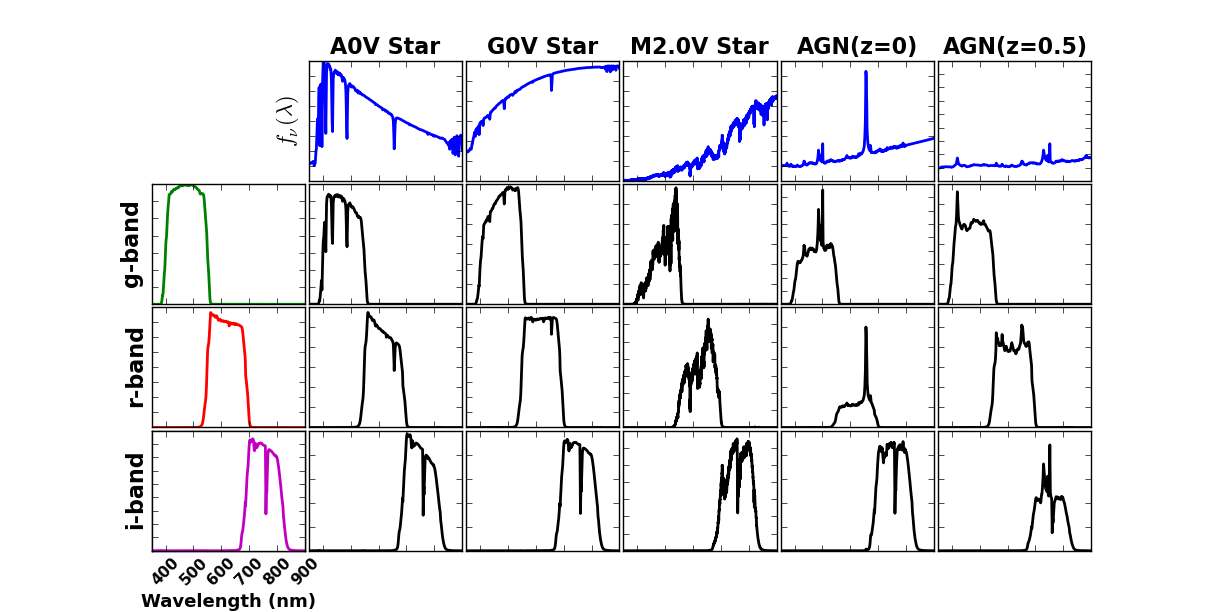
\includegraphics[width=1.1\textwidth]{\figdir/DCR1.png}
  \caption{{\bf Effective Spectral Energy Distributions} : The
    effective spectra of 5 reference objects -- a ``blue'' {\tt A0V},
    a reference {\tt G0V}, and a ``red'' {\tt M2.0V} star, along with
    a QSO at redshift $z=0$ and $z=0.5$ -- filtered through 3
    transmission profiles corresponding to the LSST $g$, $r$, and
    $i$--bands.  The top row shows the input spectral energy
    distribution $f_\nu(\lambda)$, while the leftmost column shows the
    LSST filter transmission profile in units of the normalized
    system response $\phi$.  The inner row,column figures show the
    effective spectrum of each SED (along columns) when multiplied
    through the respective filter (along rows).  In all subpanels, the
    x--axis is wavelength.  The {\tt A0V}, {\tt G0V}, and {\tt M2.0V}
    spectra correspond to {CAT\_SHARE\_DATA} files {\tt
      kp01\_9750.fits\_g45\_9830.gz}, {\tt
      km20\_6000.fits\_g30\_6020.gz}, and {\tt m2.0Full.dat.gz}
    respectively, and were used as the SEDs of the stars in the W14
    image simulations.  This figure may be recreated using the script
    {\tt python/DCR.py}.}
  \label{fig:spectra}
\end{figure}

\clearpage
\begin{figure}[h!]
  \centering
  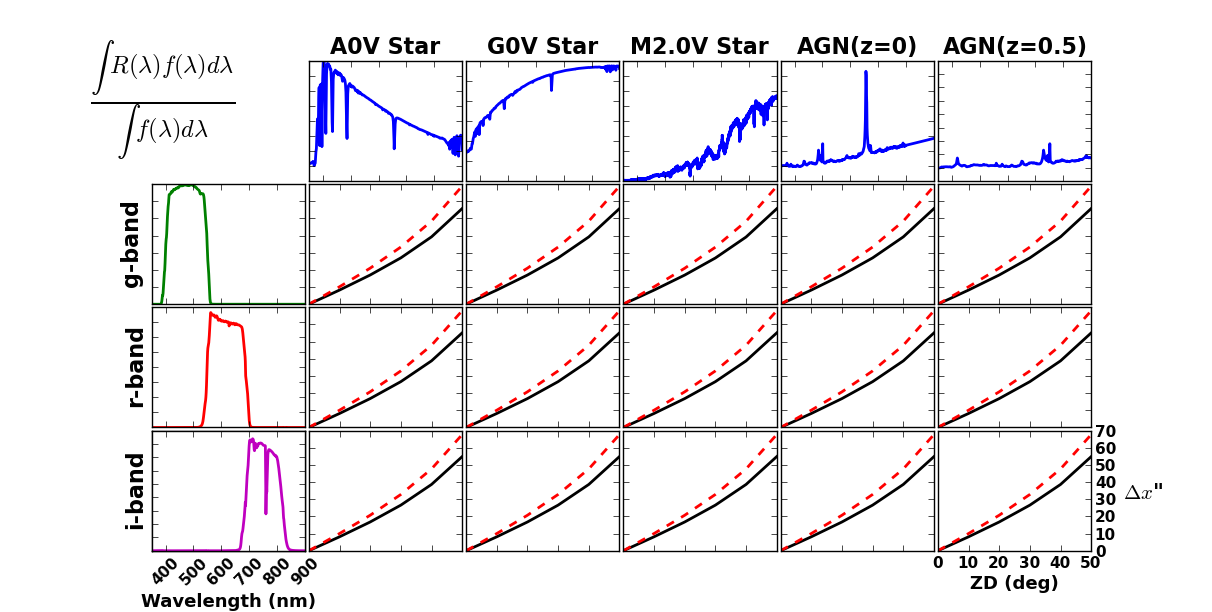
\includegraphics[width=1.1\textwidth]{\figdir/DCR2.png}
  \caption{{\bf Refraction Amplitude vs. Filter and Spectral Energy
      Distribution}: The flux-weighted amplitude of refraction (in
    arcseconds) for each of the filtered SEDs in
    Figure~\ref{fig:spectra}, as a function of zenith distance in
    degrees along the x--axis.  The solid black line is the nominal
    result from Eqn~\ref{eqn:dcr}, while the dashed red line ignores
    the corrections for temperature and pressure.  Note the maximum
    amplitude of refraction reaches nearly 1 arcminute.  This figure
    may be recreated using the script {\tt python/DCR.py}.}
  \label{fig:refraction}
\end{figure}

\clearpage
\begin{figure}[h!]
  \centering
  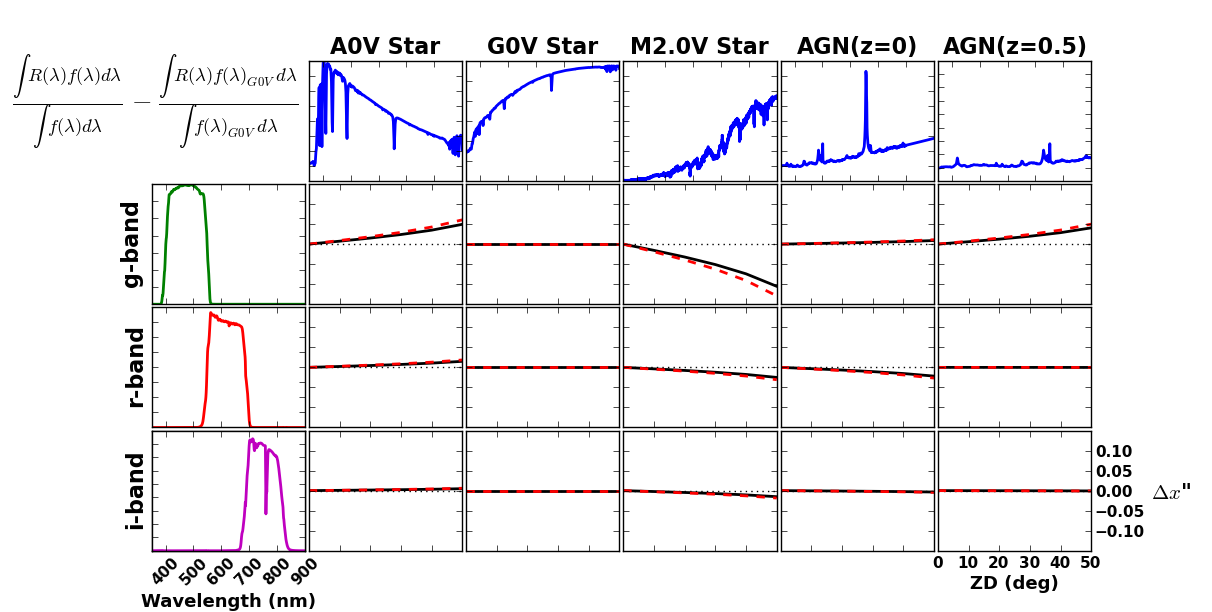
\includegraphics[width=1.1\textwidth]{\figdir/DCR3.png}
  \caption{{\bf Differential Chromatic Refraction vs. Filter and
      Spectral Energy Distribution}: The differential chromatic
    refraction of all sources from Figure~\ref{fig:spectra} with
    respect to the reference {\tt G0V} star, with respect to zenith
    distance.  The maximum amplitude of DCR reaches $0.1''$, or
    approximately half an LSST pixel.  This figure may be recreated
    using the script {\tt python/DCR.py}.}
  \label{fig:dcr}
\end{figure}

\begin{figure}[h!]
  \centering
  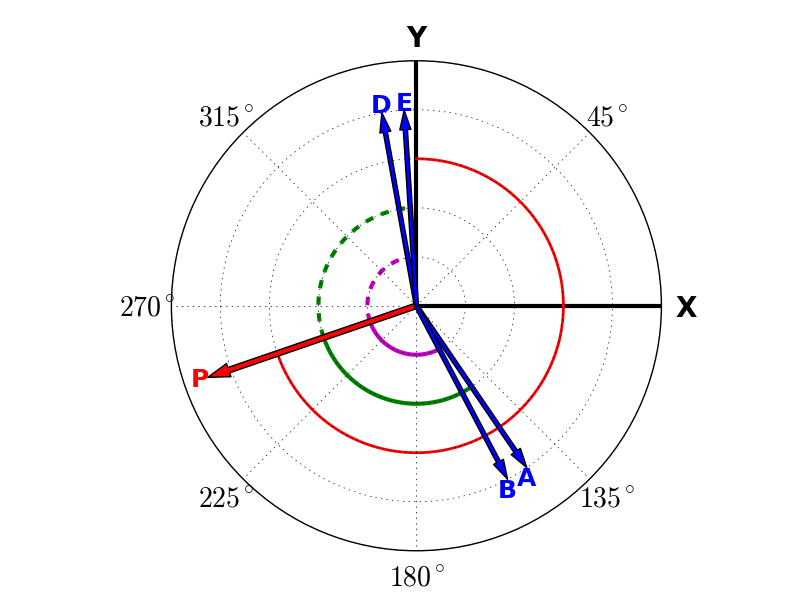
\includegraphics[width=1.1\textwidth]{\figdir/dcrPhoSim.png}
  \caption{{\bf Designed Orientation of Dcr in W14 Phosim Runs}: This
    figure represents the anticipated orientations of Dcr in the W14
    phoSim data.  The x,y coordinate system is depicted, as well as
    the convention that angles ({\tt rotTelPos}, {\tt rotSkyPos}) are
    clockwise with respect to the positive y--axis in the image
    coordinate system (counterclockwise in the camera coordinate
    system).  The {\tt rotTelPos} of 251 degrees specified for all
    simulations, which reflects the direction to the pole, is shown
    with the red vector \P and the red arc at y=0.6.  The derived {\tt
      rotSkyPos} for visits \A,\B,\D,\E\ are shown with the blue
    vectors, and reflect the angle towards zenith (the angle of
    increasing altitude).  Dcr is expected to happen along these
    vectors.  The angles \P\A,\P\E\ are similar, and represented by
    the green arcs; the angles \P\B,\P\D\ are also similar, and
    represented by the purple arcs.  This is expected as observations
    \A\ and \E\ are taken at airmass 1.55 (zenith distance of 50
    degrees) but at opposite sides of the meridian crossing of the
    star field; a similar situation was designed for observations
    \B\ and \D, which are taken at airmass 1.15 (zenith distance of 30
    degrees).  Visit \C\ is not depicted as it was taken at zenith.
    This figure was created using the script {\tt
      python/dcrSchematic.py}.}
  \label{fig:phosimdcr}
\end{figure}


\begin{figure}
    \centering
    \subfloat[Visit A]{{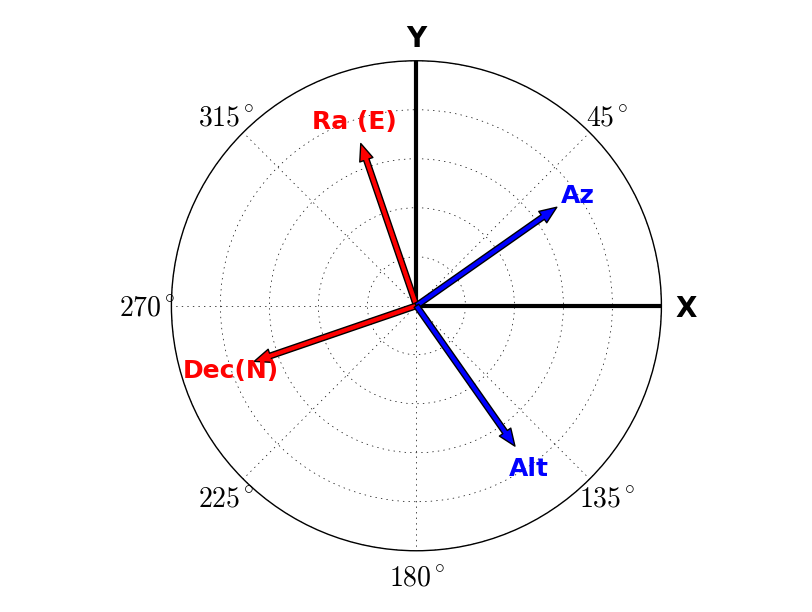
\includegraphics[width=0.46\textwidth]{\figdir/outputs8bCA_dcr_wcs.png} }}
    \qquad
    \subfloat[Visit B]{{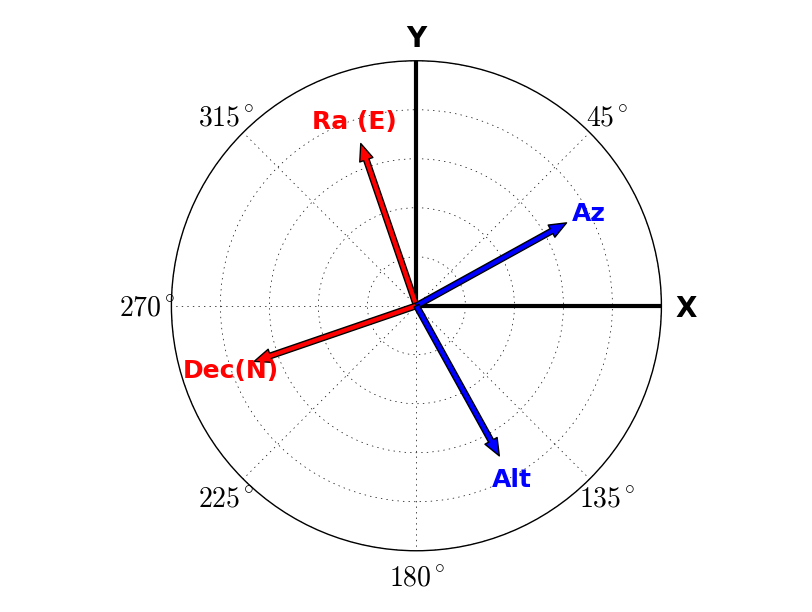
\includegraphics[width=0.46\textwidth]{\figdir/outputs8bCB_dcr_wcs.png} }} \\
    \subfloat[Visit D]{{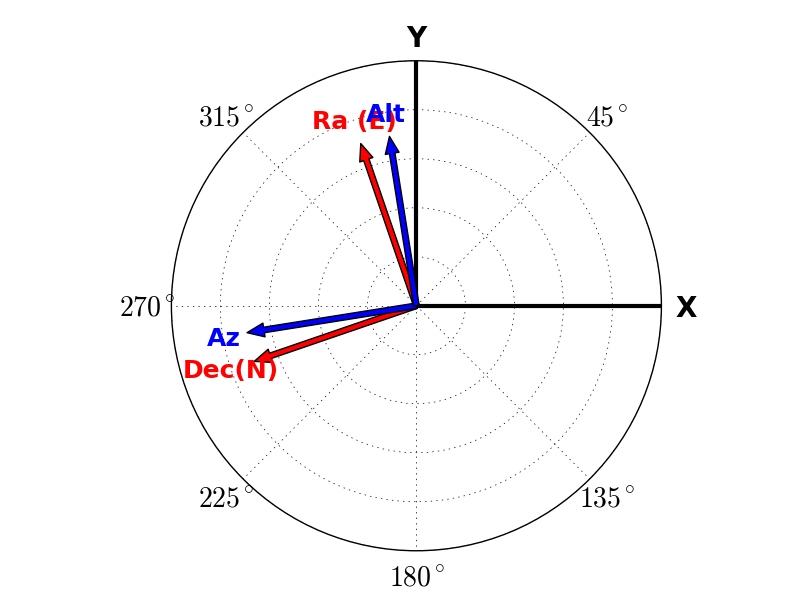
\includegraphics[width=0.46\textwidth]{\figdir/outputs8bCD_dcr_wcs.png} }}
    \qquad
    \subfloat[Visit E]{{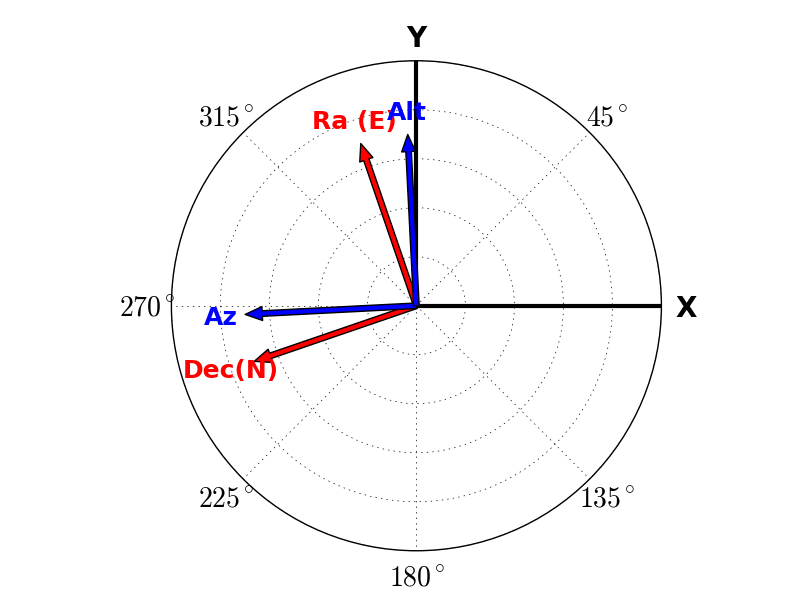
\includegraphics[width=0.46\textwidth]{\figdir/outputs8bCE_dcr_wcs.png} }} \\
    \caption{{\bf Wcs-Derived Orientations of Phosim Data}: These
      figures show the orientations of the Right Ascension and
      Declination axes (red), and Altitude and Azimuth axes (blue) of
      visits \A,\B,\D,\E.  Arrows represent the directions of {\it
        increasing} coordinate value.  The Ra,Decl axes are the same
      in all images since they were designed to have a common {\tt
        rotTelPos}.  Ideally, the directions of increasing Alt will
      correspond to the {\tt rotSkyPos} depicted in
      Figure~\ref{fig:phosimdcr}.  All coordinate system orientations
      were derived from the fitted Wcs of the {\tt calexp} of the
      $g$--band observation of seeing values {\tt 2}, i.e. the worst seeing
      image.  To determine the orientations empirically, small steps
      were taken in each coordinate starting at the center of the
      image, and the {\tt Wcs} and topocentric corrections used to map
      these back into offsets in the pixel plane.  This figure was
      created using the script {\tt python/compareDcrFromSims.py.py}.}
    \label{fig:wcsdcr}
\end{figure}

\begin{figure}[h!]
  \centering
  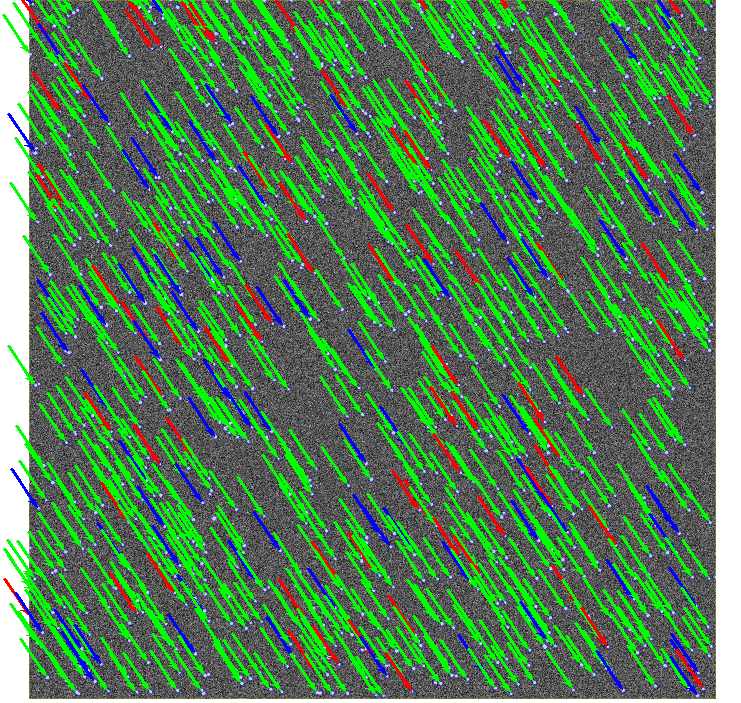
\includegraphics[width=0.5\textwidth]{\figdir/outputs8bCA_g_doPreConvolveFalse_refract_crop.png}
  \caption{{\bf Refraction}: This figure depicts the amplitude and
    orientation of the refraction vector in the visit \A, {\tt
      raft=2,2 sensor=1,1 filter=g}, seeing value {\tt 2} data.  The
    vectors point from the unrefracted locations to the realized
    locations in the image.  The SEDs of the sources are indicated
    with colors {\tt blue}, {\tt green} and {\tt red} for {\tt A0V},
    {\tt G0V}, and {\tt M2.0V} respectively.  This figure was created
    using the script {\tt python/compareDcrFromSims.py}.}
  \label{fig:refractim}
\end{figure}

\begin{figure}[h!]
  \centering
  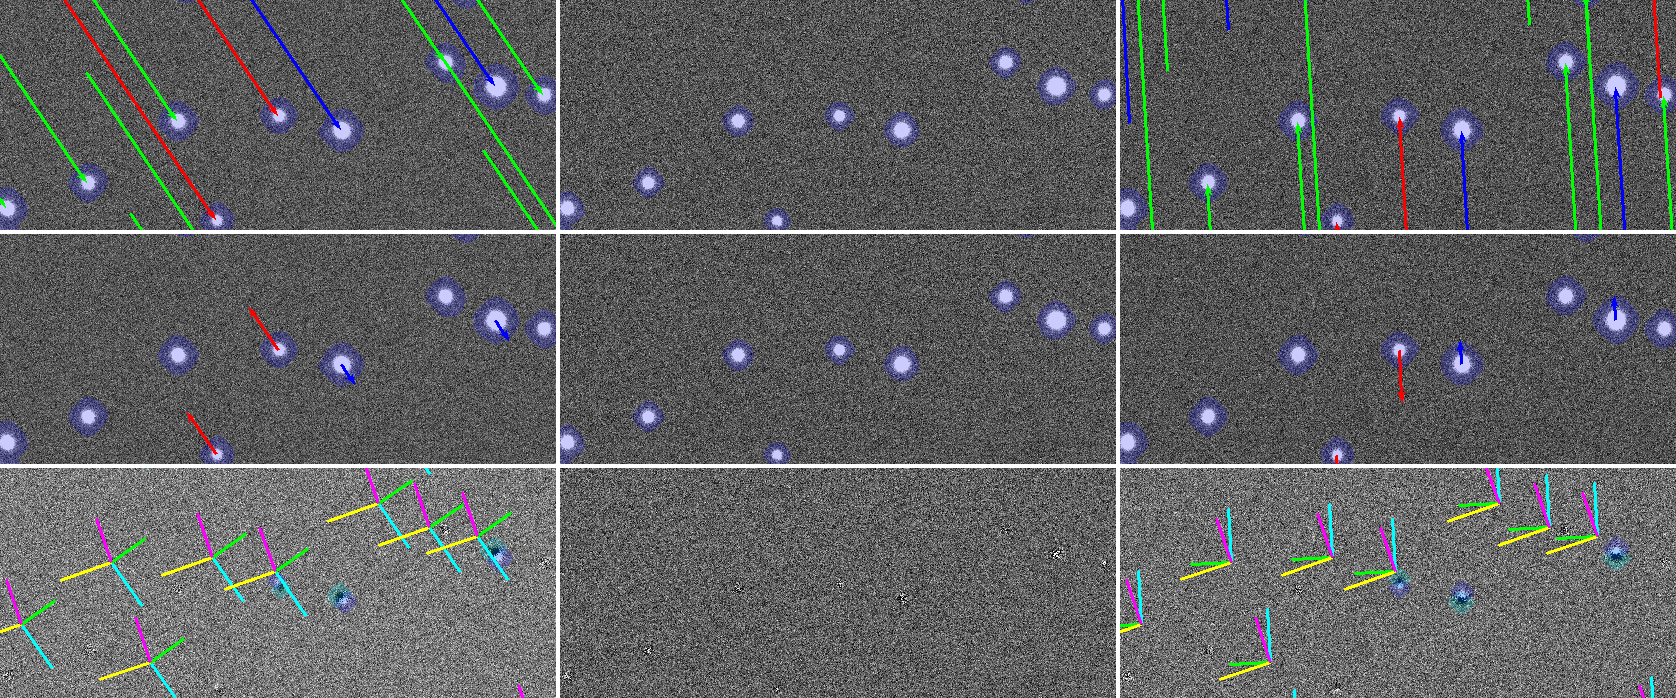
\includegraphics[width=1.0\textwidth]{\figdir/outputs8b_g_doPreConvolveFalse_dcr_crop.png}
  \caption{{\bf Differential Chromatic Refraction and Difference Image
      Quality, $g$--band}: This set of panels demonstrates the amount
    of refraction (top row), differential refraction with respect to
    the {\tt G0V} star (middle row), and the quality of the difference
    image (bottom row) for three sets of image differences.  The first
    column uses science visit \A, the middle \C, and the third \E.  In
    all cases the template used was taken at zenith, i.e. visit \C.
    The top rows effectively present the same information as
    Figure~\ref{fig:refractim}, but zoomed in on a particular cluster
    of stars.  The second row subtracts off the green vector from all
    vectors.  The residual refraction of the blue,red vectors
    represents differential chromatic refraction.  These residual
    lengths have been multiplied by a factor of 100 for readability.
    Note that the blue vectors point along the vector to zenith,
    indicating the blue stars appear higher in the sky than their
    green counterparts, compared to an unrefracted observation.  The
    red stars are not refracted as much and thus will appear lower in
    the sky.  On the bottom row, we show the realized difference image
    quality.  Note that the blue stars have positive lobes pointing
    along the direction to zenith, meaning the stars are ``higher'' in
    the sky w.r.t. the green stars when compared to the zenith
    template, while the dipoles of the red stars have the opposite
    polarity.  For completeness, the Wcs--derived orientation of the
    Ra,Decl and Az,Alt coordinate axes are shown in the difference
    image (Ra,Decl,Az,Alt are magenta,yellow,green,cyan); see
    Figure~\ref{fig:wcsdcr} for more detail.  This figure was created
    using the script {\tt python/compareDcrFromSims.py}.}
  \label{fig:dcrimg}
\end{figure}

\begin{figure}[h!]
  \centering
  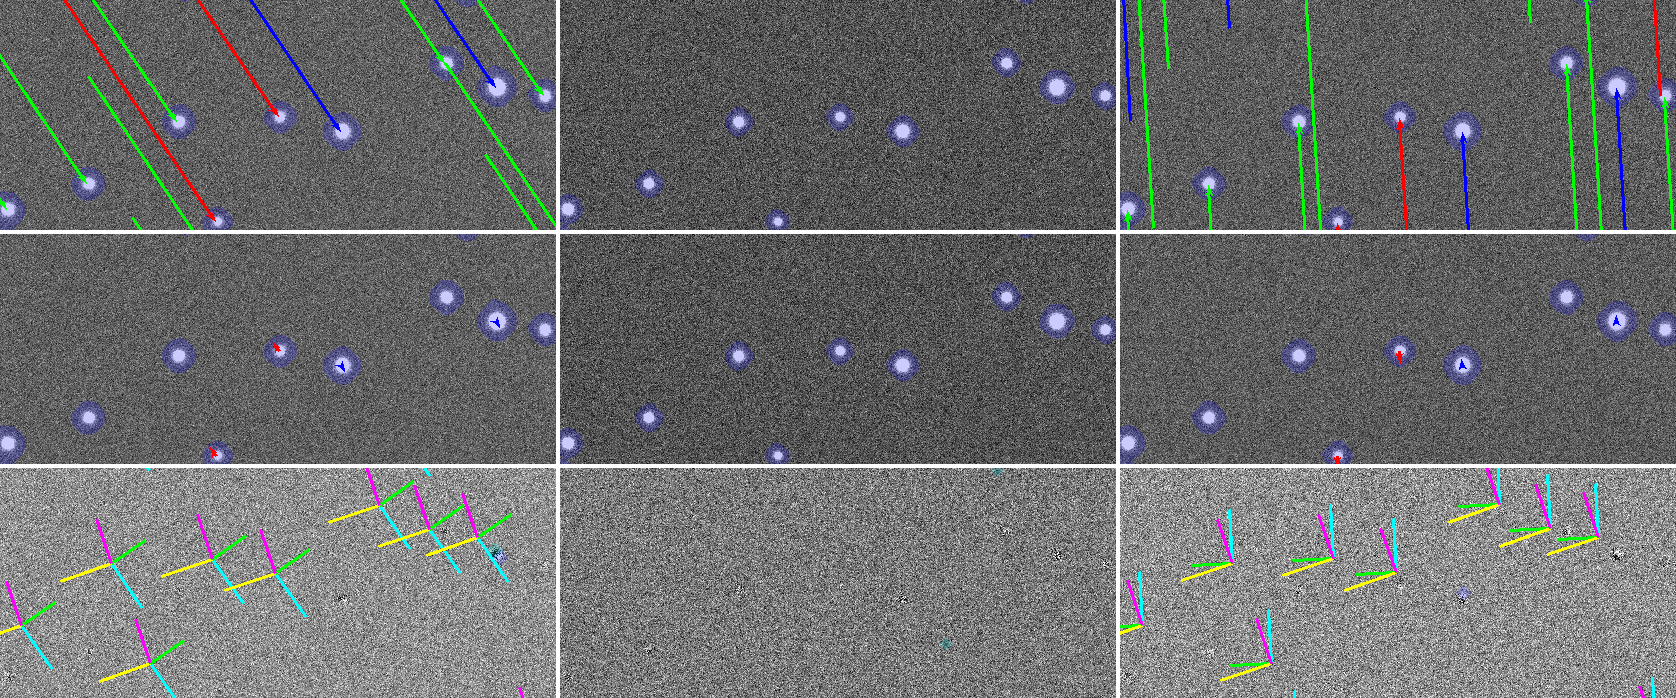
\includegraphics[width=1.0\textwidth]{\figdir/outputs8b_r_doPreConvolveFalse_dcr_crop.png}
  \caption{{\bf Differential Chromatic Refraction and Difference Image
      Quality, $r$--band}: Same as Figure~\ref{fig:dcrimg}, but for
    $r$--band data.  This figure was created using the script {\tt
      python/compareDcrFromSims.py}.}
  \label{fig:dcrimr}
\end{figure}

\begin{figure}[h!]
  \centering
  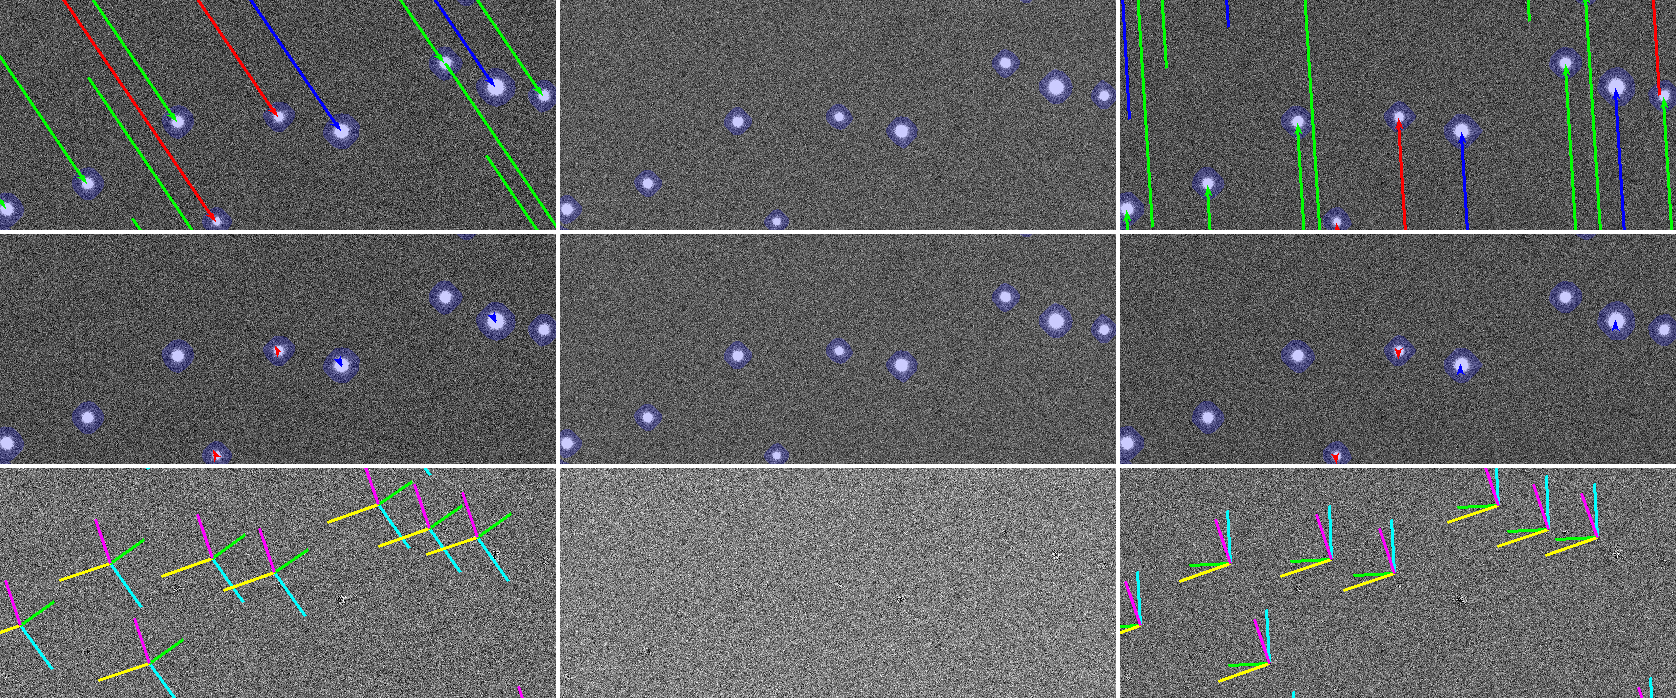
\includegraphics[width=1.0\textwidth]{\figdir/outputs8b_i_doPreConvolveFalse_dcr_crop.png}
  \caption{{\bf Differential Chromatic Refraction and Difference Image
      Quality, $i$--band}: Same as Figure~\ref{fig:dcrimg}, but for
    $i$--band data.  This figure was created using the script {\tt
      python/compareDcrFromSims.py}.}
  \label{fig:dcrimi}
\end{figure}

\begin{figure}[h!]
  \centering
  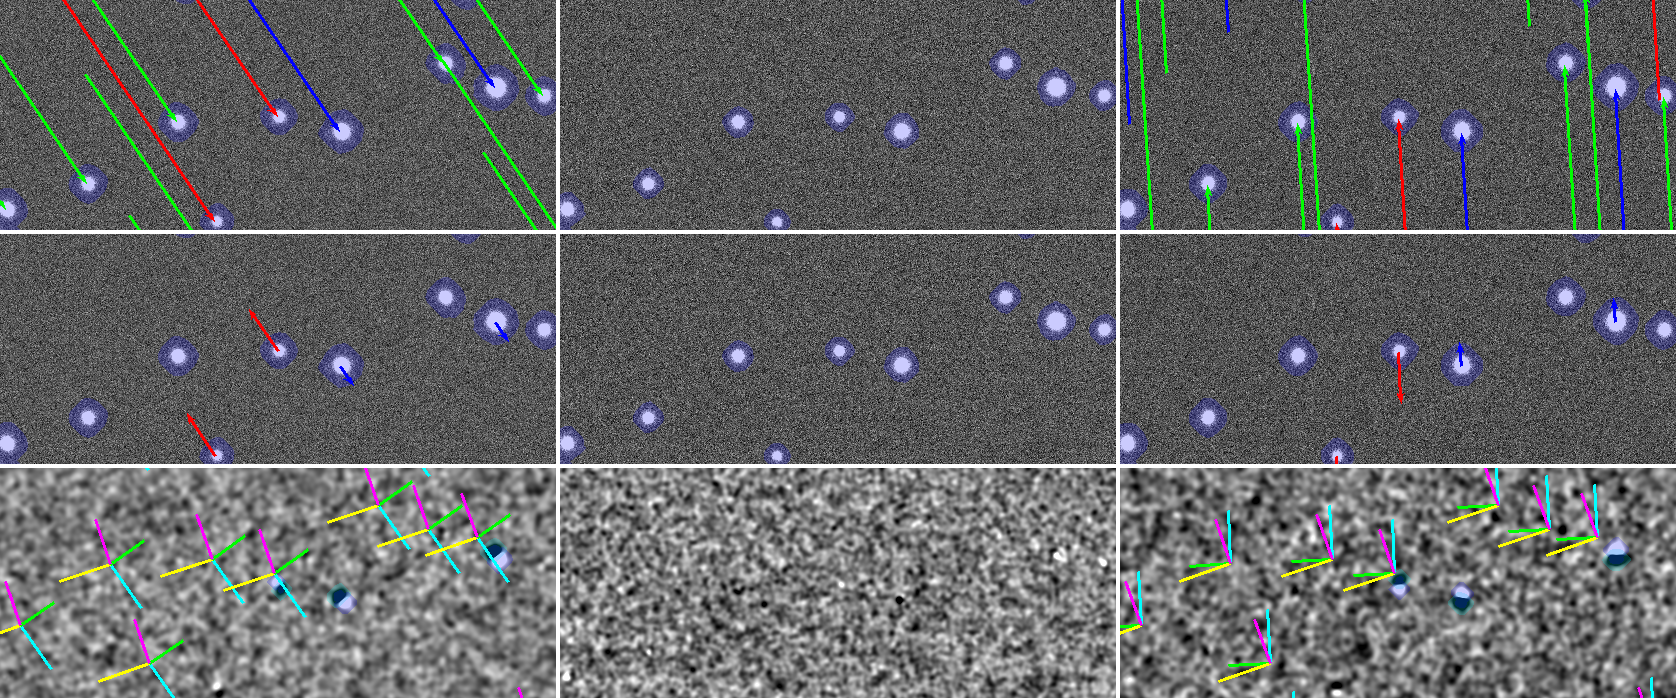
\includegraphics[width=1.0\textwidth]{\figdir/outputs8b_g_doPreConvolveTrue_dcr_crop.png}
  \caption{{\bf Differential Chromatic Refraction and Difference Image
      Quality, Prefiltering}: Same as Figure~\ref{fig:dcrimg}, but
    using prefiltering of the science image with its Psf.  This figure
    was created using the script {\tt python/compareDcrFromSims.py}.}
  \label{fig:dcrimgpre}
\end{figure}

\begin{figure}[h!]
  \centering
  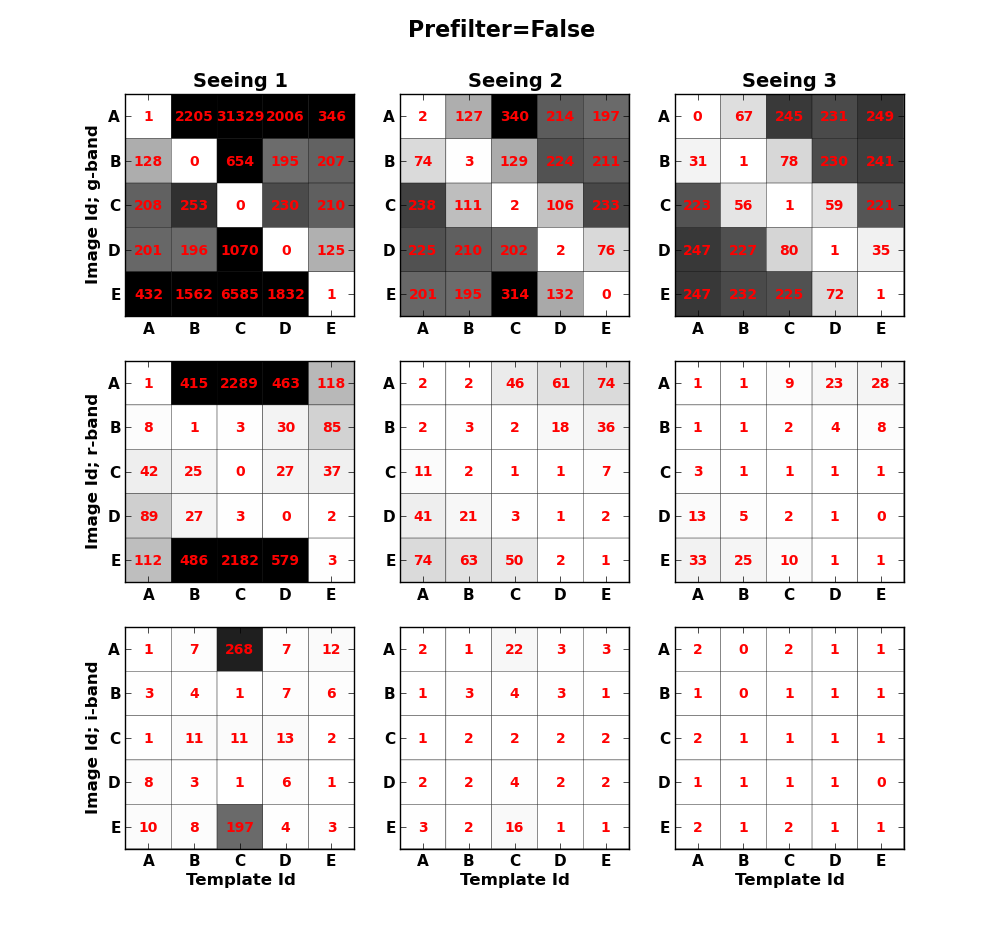
\includegraphics[width=1.0\textwidth]{\figdir/heatmapFalse.png}
  \caption{{\bf Number of False Positives, Postfiltering}: This figure
    shows the median number of false positives across the 9 {\tt
      raft=2,2} CCDs.  The first row of information shows these
    ``heat-maps'' for $g$--band data, the second for $r$--band, and
    the third for $i$--band.  The first column represents the
    good--seeing images, the second the medium--seeing images (same
    quality as template), and the third the poor-seeing images.
    Within each filter--seeing combination, the heat--map represents
    the median number of false positives as a function of the template
    airmass (visit \A\B\C\D\E) along the x--axis, and image airmass
    (visit \A\B\C\D\E) along the y--axis.  The diagonal elements
    represent the situation where the template and science image are
    taken at the same airmass and have the same orientation
    w.r.t. zenith.  The off--diagonal elements represent a mismatch
    between the template and science image in terms of airmass {\it
      and} parallactic angle.  The general trend is that the numbers
    of false positives decrease with decreasing differences in the
    airmass,angle attributes of the template and science image,
    decrease with increasing seeing, and decrease with increasing
    wavelength.  The $i$-band data in poor seeing do not appear
    sensitive to Dcr.  This figure was created using the script {\tt
      python/heatMap.py}.}
  \label{fig:heatpost}
\end{figure}

\begin{figure}[h!]
  \centering
  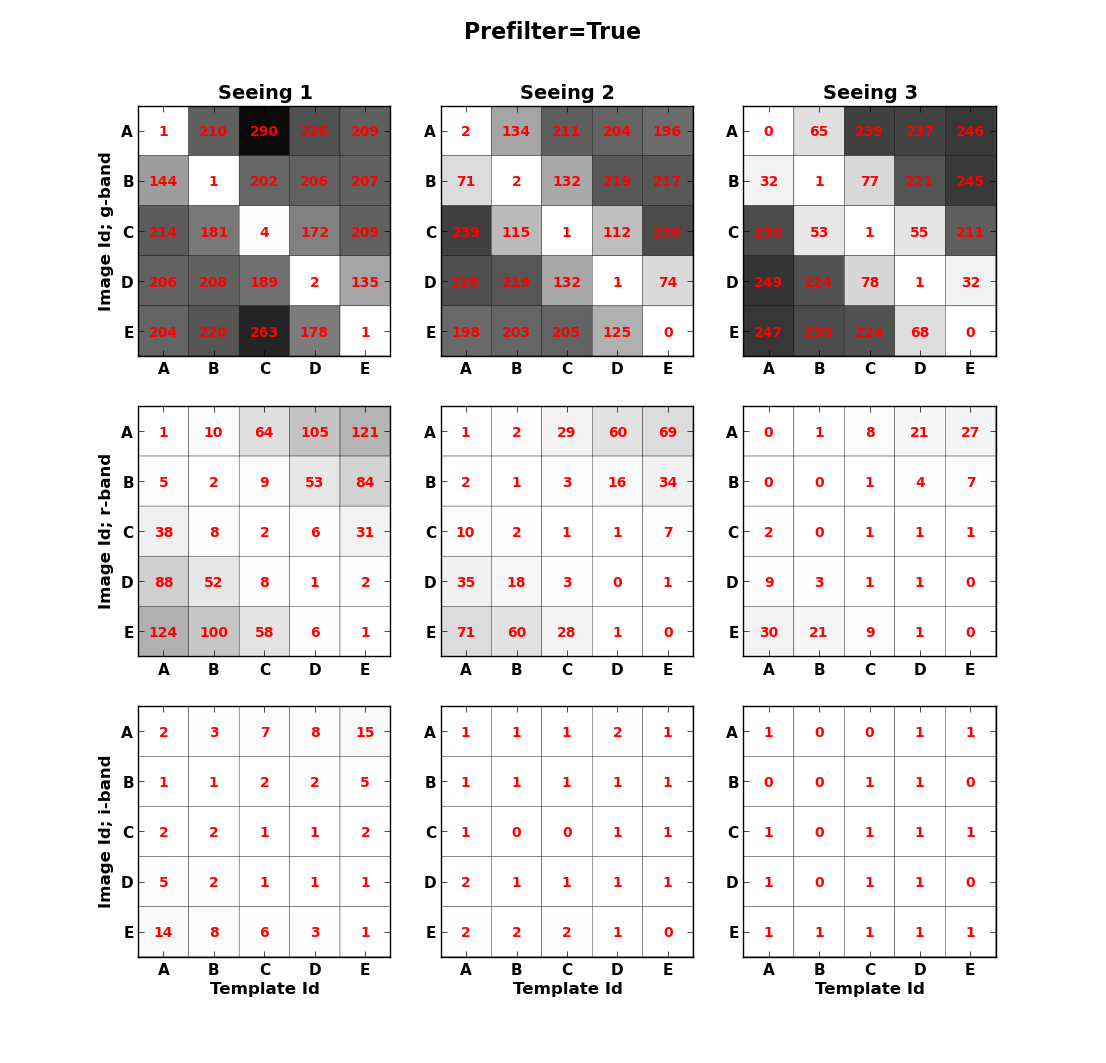
\includegraphics[width=1.0\textwidth]{\figdir/heatmapTrue.png}
  \caption{{\bf Number of False Positives, Prefiltering}: Same as
    Figure~\ref{fig:heatpost}, but using prefiltering of the science
    image with its Psf.  The numbers of false positives is overall far
    lower than in the postfiltering case (Figure~\ref{fig:heatpost}).
    This figure was created using the script {\tt python/heatMap.py}.}
  \label{fig:heatpre}
\end{figure}

%%%%%%%%%%%%%%%%%%%%%%%%% /FIGURES %%%%%%%%%%
%
%%%%%%%%%%%%%%%%%%%%%%%%% TABLES %%%%%%%%%%%%

\clearpage

\begin{table}
\centering
\begin{tabular}{cccccc}
\hline
\multicolumn{6}{|c|}{PhoSim Visits} \\
\hline
Visit & MJD           & rotSkyPos   & rotTelPos   & Altitude & Airmass \\
\hline
\A    & 51130.111719  & 251.0689567 & 145.7139810 & 40.1     & 1.55 \\
\B    & 51130.176302  & 251.0689567 & 152.2708405 & 59.9     & 1.16 \\
\C    & 51130.272830  & 251.0689567 & 341.0975816 & 89.9     & 1.00 \\
\D    & 51130.272830  & 251.0689567 & 349.8619334 & 59.9     & 1.16 \\
\E    & 51130.433247  & 251.0689567 & 356.4181128 & 40.1     & 1.55 \\
\end{tabular}
\caption[So I can have 2 paragraphs]{Summary of the configuration parameters that define each
  phoSim visit \A\B\C\D\E.  Observations were designed to follow a
  single star field through zenith on a single night, and observed
  twice before and twice after crossing the meridian, as well as at
  zenith.  Each visit was simulated using the same random seed
  (153555399), in 3 filters ($g$, $r$, $i$), and under 4 observing
  conditions.  These correspond to the template image ({\tt
    Opsim\_rawseeing} = 0.878'' and {\tt SIM\_VISTIME} = 300) and then
  3 bins in seeing for the science image corresponding to {\tt
    Opsim\_rawseeing} = 0.6'', 0.878'', and 1.2'' for seeing bins {\tt
    1,2,3}, respectively.  All science images were simulated with {\tt
    SIM\_VISTIME} = 15.  
  \\ ~ \\
  Overall, this yielded $5 \times 3 \times 4 = 60$ runs of phoSim,
  which are encoded as {\tt visitId=X00Y00Z} where {\tt X} represents
  the phoSim filterId $gri$={\tt 123}, {\tt Y} represents the visit
  \A\B\C\D\E = {\tt 01234}, and {\tt Z} represents the seeing:
  {\tt 0} for the template and {\tt 123} for the science
  images.  All 9 CCDs within {\tt raft=2,2} were simulated.
  All trim files used to generate the sims for this
  analysis may be found in the {\tt sims8/} directory.}
\label{tab:visits}
\end{table}

\begin{table}
\centering
\begin{tabular}{ccccc}
\hline
\multicolumn{5}{|c|}{Orientation of Dcr} \\
\hline
Visit    & SED & {\tt rotTelPos} & {\tt Wcs} + Topo & Measured \\
         &     &                 &                  & Dipole Orientation \\
\hline
\A & {\tt A0V}   & $145.7^{\circ}$ & $144.9^{\circ}$ & $145.7^{\circ}$    \\
   & {\tt M2.0V} & $325.7^{\circ}$ & $324.9^{\circ}$ & $325.6^{\circ}$    \\
\hline
\B & {\tt A0V}   & $152.3^{\circ}$ & $151.1^{\circ}$ & $151.7^{\circ}$    \\
   & {\tt M2.0V} & $332.3^{\circ}$ & $331.1^{\circ}$ & $331.8^{\circ}$    \\
\hline
\D & {\tt A0V}   & $349.9^{\circ}$ & $351.0^{\circ}$ & $349.3^{\circ}$    \\
   & {\tt M2.0V} & $169.9^{\circ}$ & $171.0^{\circ}$ & $170.0^{\circ}$    \\
\hline
\E & {\tt A0V}   & $356.4^{\circ}$ & $357.1^{\circ}$ & $355.2^{\circ}$    \\
   & {\tt M2.0V} & $176.4^{\circ}$ & $177.1^{\circ}$ & $176.2^{\circ}$    \\
\end{tabular}
\caption[So I can have 2 paragraphs]{The expected and measured
  orientations of Dcr, using the coordinate conventions depicted in
  Figure~\ref{fig:phosimdcr}.  These numbers represent the orientation
  of the {\it positive} lobe of any dipole arising from the Dcr
  effect.  Numbers are reported as a function of visit \A--\E, and the
  spectral energy distribution of the source.  For the {\tt rotTelPos}
  and {\tt Wcs} columns, the numbers for the red {\tt M2.0V} stars are
  simply $180^{\circ}$ from those of the blue {\tt A0V} stars, which
  should be in the direction of zenith.  The numbers under {\tt
    rotTelPos} reflect the designed orientation of Dcr that was input
  to phoSim.  The numbers under {\tt Wcs} reflect the empirically
  determined direction to zenith in each image, using the {\tt calexp}
  fitted {\tt Wcs} and topocentric corrections appropriate for each
  visit.  Finally, we report the measured median orientation of
  DiaSources in each image difference, when differenced against the
  template taken at zenith (visit \C).  Here the red and blue
  populations are considered separately.  \\ ~ \\ These numbers come
  from analysis of $g$--band data, seeing bin {\tt 1}, which have the
  most dipoles.  We only show results for 1 filter since the
  orientation should be filter--independent.  Results in the
  $r$--band, in cases where there are more than 10 dipoles measured,
  show quantitatively similar results.  In addition, we only report
  numbers from the postfiltered data, where dipole measurement is
  known to operate correctly.  We do not see any dependence of these
  orientations on the seeing.  Full results may be found in the file
  {\tt NOTES}.}
\label{tab:dcrang}
\end{table}

\begin{table}
\centering
\begin{tabular}{cccccccc}
\hline
\multicolumn{8}{|c|}{Amplitude of Dcr} \\
\hline
Visit    & SED & Filter & Theory & {\tt Wcs} Offsets & Dipole Amplitude   & Dipole Amplitude   & Dipole Amplitude \\
         &     &        &        &                   & Seeing Bin {\tt 1} & Seeing Bin {\tt 2} & Seeing Bin {\tt 3} \\
\hline
\A & {\tt A0V}   & $g$ & 0.049'' & 0.042'' & 0.167''  & 0.259''  & 0.208''  \\
   &             & $r$ & 0.015'' & 0.013'' & 0.049''  & $\cdots$ & $\cdots$ \\
   &             & $i$ & 0.005'' & 0.005'' & $\cdots$ & $\cdots$ & $\cdots$ \\
   & {\tt M2.0V} & $g$ & 0.105'' & 0.077'' & 0.144''  & 0.204''  & 0.293''  \\
   &             & $r$ & 0.025'' & 0.020'' & 0.230''  & $\cdots$ & $\cdots$ \\
   &             & $i$ & 0.015'' & 0.012'' & $\cdots$ & $\cdots$ & $\cdots$ \\
\hline
\B & {\tt A0V}   & $g$ & 0.024'' & 0.020'' & 0.183''  & 0.243''  & $\cdots$ \\
   &             & $r$ & 0.007'' & 0.006'' & $\cdots$ & $\cdots$ & $\cdots$ \\
   &             & $i$ & 0.002'' & 0.002'' & $\cdots$ & $\cdots$ & $\cdots$ \\
   & {\tt M2.0V} & $g$ & 0.051'' & 0.038'' & 0.222''  & 0.266''  & $\cdots$ \\
   &             & $r$ & 0.012'' & 0.010'' & $\cdots$ & $\cdots$ & $\cdots$ \\
   &             & $i$ & 0.007'' & 0.005'' & $\cdots$ & $\cdots$ & $\cdots$ \\
\hline
\D & {\tt A0V}   & $g$ & 0.024'' & 0.020'' & 0.201''  & 0.251''  & $\cdots$ \\
   &             & $r$ & 0.007'' & 0.006'' & $\cdots$ & $\cdots$ & $\cdots$ \\
   &             & $i$ & 0.002'' & 0.002'' & $\cdots$ & $\cdots$ & $\cdots$ \\
   & {\tt M2.0V} & $g$ & 0.051'' & 0.038'' & 0.201''  & 0.254''  & $\cdots$ \\
   &             & $r$ & 0.012'' & 0.010'' & $\cdots$ & $\cdots$ & $\cdots$ \\ 
   &             & $i$ & 0.007'' & 0.006'' & $\cdots$ & $\cdots$ & $\cdots$ \\
\hline
\E & {\tt A0V}   & $g$ & 0.049'' & 0.042'' & 0.169''  & 0.235''  & 0.360''  \\
   &             & $r$ & 0.015'' & 0.013'' & 0.135''  & $\cdots$ & $\cdots$ \\
   &             & $i$ & 0.005'' & 0.005'' & $\cdots$ & $\cdots$ & $\cdots$ \\
   & {\tt M2.0V} & $g$ & 0.105'' & 0.077'' & 0.158''  & 0.213''  & 0.267''  \\
   &             & $r$ & 0.025'' & 0.020'' & 0.262''  & $\cdots$ & $\cdots$ \\
   &             & $i$ & 0.015'' & 0.011'' & $\cdots$ & $\cdots$ & $\cdots$ \\
\end{tabular}
\caption[So I can have 2 paragraphs]{The expected and measured
  amplitudes of Dcr, in arcseconds.  These numbers represent the
  differential offset between positions of an object at zenith (visit
  \C) and at the airmasses associated with visits \A\B\D\E, with
  respect to the positions of the reference {\tt G0V} stars, which
  define the astrometric reference system in this study.  The Theory
  column is the expected amplitude as described in
  Section~\ref{sec:theory}, using the reference SEDs described in
  Section~\ref{sec:seds}.  The {\tt Wcs} column represents the mean
  offsets between stars of the given SED and the astrometric reference
  solution, determined using {\tt calexp's} {\tt Wcs} and {\tt Source}
  products.  Residuals of the reference {\tt G0V} stars are smaller
  than 0.002'' in all cases.  The dipole amplitudes are determined
  using the same fits that yield the dipole orientations in
  Table~\ref{tab:dcrang}, and represent the offset between the fitted
  positive and negative lobes of the dipole.  These numbers are only
  reported for data sets that contain more than 10 measurements.
  Because we see a seeing dependence on these numbers, we report them
  for each of the seeing bins {\tt 1,2,3}.  Full results may be found
  in the file {\tt NOTES}.}
\label{tab:dcramp}
\end{table}

%%%%%%%%%%%%%%%%%%%%%%%%% /TABLES %%%%%%%%%%%


\clearpage
\bibliographystyle{apj}
\bibliography{refs}

\clearpage
\begin{appendices}
\section{Use of PhoSim}

I describe here the end-to-end process of generating instance (or
trim) files for {\tt phoSim}, running these images to create output
{\tt eImages}, creating {\tt astrometry.net} index files for
astrometric calibration, and running these images through {\tt
  processEimage.py}.  This does {\it not} include the process of
generating instance catalogs from a master base catalog, or the
process of using calibration data to run the simulated images through
{\tt processCcd.py}, which does (amongst other operations) the
assembly of amp images into CCD images and instrument signature
removal.  The process is described for {\tt phoSim} version 3.3.2.

\subsection{Setting up PhoSim}

\subsection{Generation of Instance Catalogs for W14 \label{appx:tasks}}

\subsubsection{General}
exposure times
single snap
control file
header
seeing

\subsubsection{Subtask 1}

We describe our first step in the {\tt phoSim} process, the generation
of the input configuration.  We start with the trim files used in W13
processing, which consist of a random star field populated by stars of
SED {\tt km50\_5000.fits\_g20\_5140.gz}, and covering a range of
magnitudes $19 < r < 21$.  Observations were designed to be at a
zenith distance of $20.2^{\circ}$, with a boresight pointing of (Ra,
Decl) = ($79.68926^{\circ}, -9.70229^{\circ}$).  Observations were
simulated in the $i$--band.  These trim files are stored in the {\tt sims3/}
directory in this repository.

\subsubsection{Subtask 2}

We chose spectrum {\tt km20\_6000.fits\_g30\_6020.gz} for our
reference {\tt G0V}-star, and replaced 80\% of the objects in the
original trim file with this SED.  We then selected the bluest object
contained in the base catalog, {\tt kp01\_9750.fits\_g45\_9830.gz},
for every tenth object starting at object \#0, and the most populous
red object in the catalog {\tt m2.0Full.dat.gz} for every tenth object
starting at object \#5.  These correspond to spectral types {\tt A0V}
and {\tt M2.0V}, respectively.  

Because the magnitudes in the trim files represent a 500nm magnitude
(approximate $g$--band), it was required to make color corrections to
the requested magnitudes of the objects to preserve the relative
brightness distribution of the as--simulated, multi--SED sources.
This was done using their respective $i$--band magnitudes (i.e. a
correction of $-2.5~log_{10}~( f_{i;SED} / f_{i;GOV} )$).
Accordingly, the brightness distributions in the $gr$--bands were not
optimal (this was fixed in Task C).  The colors of each spectral type
were calculated using {\tt python/colors.py}.  Script {\tt
  makeNewTrims.py} was used to make these modifications to the {\tt
  sims3/} trim files, yielding {\tt sims5/} trim files ($i$--band).
The only modifications made to the input trim files to simulate images
in the $gr$--bands were to change the {\tt Opsim\_filter} field to
indicate $gri$ = 123; these are stored in the {\tt sims5gr/}
directory.

\subsubsection{Subtask 3}

First, to have similar brightness distributions in all data, we make a
SED--dependent {\it and} passband--dependent magnitude correction to
the trim files used for this task.  These corrections are made in
script {\tt generateTrimFilesDcr.py}, which ran on the $i$--band trim
files from {\tt sims5}.

Second, the original observations do not pass through zenith on the
given night of simulated observations.  To design the observations to
pass through zenith at the LSST site, which is at southern latitude
$-29.67^{\circ}$, we first subtracted $19.96437^{\circ}$ from all
coordinates in the input trim files so that the field is centered at a
declination equal to the Southern latitude of the site.  This includes
both the per-object coordinates and the boresight pointing {\tt
  Unrefracted\_Dec} in the trim file header.

We simulated this star field throughout the night of MJD 51130 (the
night of the fiducial image simulations) to establish the times at
which it was at an altitude of 40 and 60 degrees (zenith distance of
50 and 30 degrees; airmass of 1.55 and 1.15), and when it was closest
to zenith.  We chose 5 specific times at which to simulate the images:
before meridian crossing at airmass 1.55; before meridian crossing at
airmass 1.15; closest to zenith; after meridian crossing at airmass
1.15; after meridian crossing at airmass 1.55).

Because the instance catalog inputs to {\tt phoSim} form an
overcomplete set (e.g. the user specifies Ra, Decl, altitude, azimuth,
and time of observation), it is possible to request a simulation
configuration that is not physically possible.  For this reason, we
used \\{\tt
  lsst.sims.catalogs.measures.example\_utils.makeObsParamsRaDecSky}
subroutine \\{\tt makeObsParamsRaDecSky} to generate a self--consistent
set of observation parameters given the Ra and Decl of the field, and
the times of observation established above.

In addition, this script synchronized the values of {\tt
  Opsim\_rotskypos} and {\tt Opsim\_rottelpos}.  {\tt Rotskypos} sets
the orientation of Ra and Decl of the catalog, effectively a rotation
of the Pole away from the Zenith.  When {\tt rotskypos=0} the Ra
direction is ``up'', along the y--axis.  This value was kept the same
for all images, so that the star field was always rendered in
approximately the same orientation.  {\tt Rottelpos} is defined as
({\tt rotskypos}-180+parallactic angle), such that the angle of DCR
should be along this axis.  This will also be the angle of increasing
Altitude in the Az,Alt coordinate system.  This value is observation
dependent, and was determined using {\tt makeObsParamsRaDecSky}.  Trim
files for this run are found in the {\tt sims8/} directory of this
repository.

\subsection{Running {\tt phosim.py}}

\subsection{Creating Astrometry Index Files}

setup -r /lsst/home/krughoff/lsst/lsst\_devel/Linux64/astrometry.net-0.38/astrometry
text2fits.py 2002000.ref 2002000.fits
setenv P 1402120
build-index -i 2002000.fits -o index-${P}00.fits -I ${P}00 -P 0 -S r -n 100 -L 20 -E -j 0.4 -r 1
build-index -1 index-${P}00.fits -o index-${P}01.fits -I ${P}01 -P 1 -S r -L 20 -E -M -j 0.4 
build-index -1 index-${P}00.fits -o index-${P}02.fits -I ${P}02 -P 2 -S r -L 20 -E -M -j 0.4 
build-index -1 index-${P}00.fits -o index-${P}03.fits -I ${P}03 -P 3 -S r -L 20 -E -M -j 0.4 
build-index -1 index-${P}00.fits -o index-${P}04.fits -I ${P}04 -P 4 -S r -L 20 -E -M -j 0.4 
ls index-1402120* | awk '{printf("modhead %s+7 REFCAT '2002000'\n",\$1)}' | sh     
setup astrometry\_net 0.30  
cp -r /nfs/lsst/home/becker/Winter2014/astrometry\_net\_data/ups .
edit andConfig.py 
setup -k -r .

\subsection{Running processEimage.py}

\section{ImageDifferenceTask}


We used {\tt \$PIPE\_TASKS\_DIR/bin/imageDifferenceWinter2013.py},
which has an additional flag that allows us to use a particular visit
ID as the template, instead of extracting one from the template
archive.

\end{appendices}

\end{document}
